\begin{example}[Définition 1 : $n = 7$]
    ~
    \begin{itemize}
        \item $f_1 = (7, 3, 1, 4, 2, 5, 2) \in \mathcal{PF}_7$
        \item $f_2 = (7, 3, 1, 4, 2, 5, 4) \notin \mathcal{PF}_7$
    \end{itemize}
\end{example}

\begin{example}[Théorème 2 : $n = 3 : pf_3 = 16$]
    ~\\
    \begin{itemize*}             
        \item $(1, 1, 1)$
        \item $(1, 1, 2)$
        \item $(1, 1, 3)$
        \item $(1, 2, 1)$
        \item $(1, 2, 2)$
        \item $(1, 2, 3)$
        \item $(1, 3, 1)$
        \item $(1, 3, 2)$
        \item $(2, 1, 1)$
        \item $(2, 1, 2)$
        \item $(2, 1, 3)$
        \item $(2, 2, 1)$
        \item $(2, 3, 1)$
        \item $(3, 1, 1)$
        \item $(3, 1, 2)$
        \item $(3, 2, 1)$
    \end{itemize*}
\end{example}

\begin{example}[Définition 3 : $n = 4$]
    ~
    \begin{itemize}
        \item $f_1 = (1, 2, 2, 3) \in \mathcal{PF'}_4$
        \item $f_2 = (1, 2, 3, 2) \notin \mathcal{PF'}_4
         \text{, bien que } f_2 \in \mathcal{PF}_4$
    \end{itemize}
\end{example}

\begin{example}[Théorème 4 : $n = 3 : pf'_3 = 5$]
    ~\\
    \begin{itemize*}
        \item $(1, 1, 1)$
        \item $(1, 1, 2)$
        \item $(1, 1, 3)$
        \item $(1, 2, 2)$
        \item $(1, 2, 3)$
    \end{itemize*}
\end{example}

\begin{example}[Définition 5 : $n = 5$]
    ~
    \begin{itemize}
        \item $w_1 = 1011000110 \text{ n'est \emph{pas} un mot de Dyck,
        car } |1011000|_0 > |1011000|_1.$
        \item $w_2 = 1011010101 \text{ n'est \emph{pas} un mot de Dyck,
        car } |w_2|_0 \neq |w_2|_1.$
        \item $w_3 = 1011010100 \text{ \emph{est} un mot de Dyck : }$
    \end{itemize}
    ~\\
\begin{center}
    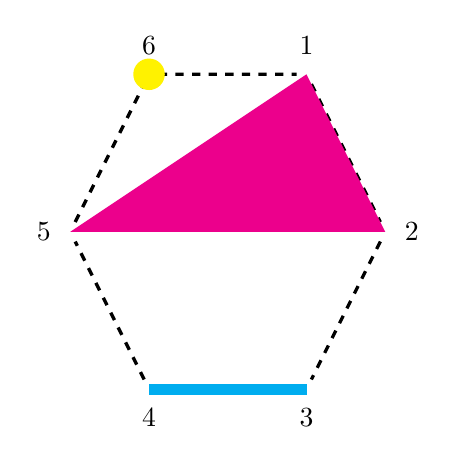
\begin{tikzpicture}[scale=1]
        \node [label = above : {$1$}] (1)
            at (4,5) {};
        \node [label = right : {$2$}] (2)
            at (5,3) {};
        \node [label = below : {$3$}] (3)
            at (4,1) {};
        \node [label = below : {$4$}] (4)
            at (2,1) {};
        \node [label = left : {$5$}]  (5)
            at (1,3) {};
        \node [label = above : {$6$}] (6)
            at (2,5) {};
        \draw [dashed][very thick]
        (1) -- (2) -- (3) -- (4)
            -- (5) -- (6) -- (1);
        \fill [color = magenta] (4,5) -- (5,3)
            -- (1,3) -- cycle;
        \draw [color = cyan][line width = 4pt] 
            (4,1) -- (2,1);
        \fill [color=yellow] (2,5) circle (0.2);
      \end{tikzpicture}
\end{center}
\end{example}

\begin{example}[Théorème 6 : $n = 3$]
    $d_3 = 5$.
    \begin{center}
        \begin{center}
    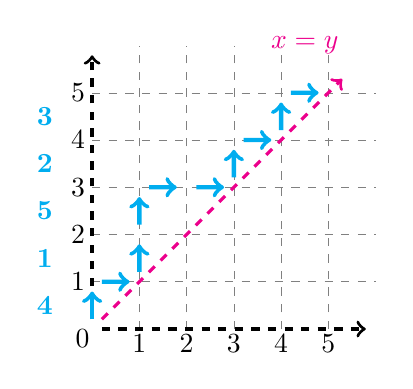
\begin{tikzpicture}[scale=0.6]
        \node (a) at (0, 0) {};
        \node (b) at (0, 6) {};
        \node (c) at (6, 0) {};
        \node (d) at (5.5, 5.5) {};

        \draw [dashed, very thin, color=gray] (1,0) to (1,6);
        \draw [dashed, very thin, color=gray] (2,0) to (2,6);
        \draw [dashed, very thin, color=gray] (3,0) to (3,6);
        \draw [dashed, very thin, color=gray] (4,0) to (4,6);
        \draw [dashed, very thin, color=gray] (5,0) to (5,6);
        \draw [dashed, very thin, color=gray] (0,1) to (6,1);
        \draw [dashed, very thin, color=gray] (0,2) to (6,2);
        \draw [dashed, very thin, color=gray] (0,3) to (6,3);
        \draw [dashed, very thin, color=gray] (0,4) to (6,4);
        \draw [dashed, very thin, color=gray] (0,5) to (6,5);

        \node (e) at (4.5, 6) [color = magenta] {$x = y$}; 
        \draw [dashed, very thick, ->] (a) to (b);
        \draw [dashed, very thick, ->] (a) to (c);
        \draw [dashed, very thick, ->]
            [color = magenta] (a) to (d);

        \node (1)  at (0,0)   {};
        \node (2)  at (0,1)   {};
        \node (3)  at (1,1)   {};
        \node (4)  at (1,2)   {};
        \node (5)  at (1,3)   {};
        \node (6)  at (2,3)   {};
        \node (7)  at (3,3)   {};
        \node (8)  at (3,4)   {};
        \node (9)  at (4,4)   {};
        \node (10) at (4,5)   {};
        \node (11) at (5,5)   {};
        \draw [->, ultra thick, color = cyan]
            (1)  to (2);
        \draw [->, ultra thick, color = cyan] 
            (2)  to (3);
        \draw [->, ultra thick, color = cyan]
            (3)  to (4);
        \draw [->, ultra thick, color = cyan]
            (4)  to (5);
        \draw [->, ultra thick, color = cyan]
            (5)  to (6);
        \draw [->, ultra thick, color = cyan]
            (6)  to (7);
        \draw [->, ultra thick, color = cyan]
            (7)  to (8);
        \draw [->, ultra thick, color = cyan]
            (8)  to (9);
        \draw [->, ultra thick, color = cyan]
            (9)  to (10);
        \draw [->, ultra thick, color = cyan]
            (10) to (11);

        \node at (-0.2, -0.2) {$0$};
        \node at (-0.3, 1)    {$1$};
        \node at (1, -0.3)    {$1$};
        \node at (-0.3, 2)    {$2$};
        \node at (2, -0.3)    {$2$};
        \node at (-0.3, 3)    {$3$};
        \node at (3, -0.3)    {$3$};
        \node at (-0.3, 4)    {$4$};
        \node at (4, -0.3)    {$4$};
        \node at (-0.3, 5)    {$5$};
        \node at (5, -0.3)    {$5$};

        \node [color = cyan] at (-1, 0.5) {\textbf{4}};
        \node [color = cyan] at (-1, 1.5) {\textbf{1}};
        \node [color = cyan] at (-1, 2.5) {\textbf{5}};
        \node [color = cyan] at (-1, 3.5) {\textbf{2}};
        \node [color = cyan] at (-1, 4.5) {\textbf{3}};

    \end{tikzpicture}
\end{center}
    \end{center}
\end{example}

\begin{example}[Définition 7 : $n = 5$]
    ~
    \begin{itemize}
        \item $w_1 = 4051002030 \text{ n'est \emph{pas} un mot de Dyck
            décoré, car } 5 > 1.$
        \item $w_2 = 4015002030 \text{ \emph{est} un mot de Dyck décoré :}$
    \end{itemize}
    \begin{center}
    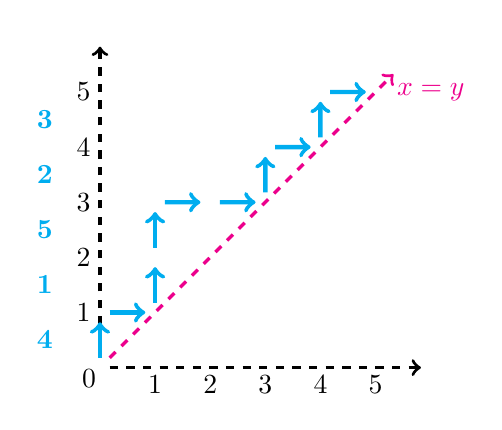
\begin{tikzpicture}[scale=0.7]
        \node (a) at (0, 0) {};
        \node (b) at (0, 6) {};
        \node (c) at (6, 0) {};
        \node (d) at (5.5, 5.5) {};
        \node (e) at (6, 5) [color = magenta]
            {$x = y$}; 
        \draw [dashed, very thick, ->] (a) to (b);
        \draw [dashed, very thick, ->] (a) to (c);
        \draw [dashed, very thick, ->]
            [color = magenta] (a) to (d);

        \node (1)  at (0,0)   {};
        \node (2)  at (0,1)   {};
        \node (3)  at (1,1)   {};
        \node (4)  at (1,2)   {};
        \node (5)  at (1,3)   {};
        \node (6)  at (2,3)   {};
        \node (7)  at (3,3)   {};
        \node (8)  at (3,4)   {};
        \node (9)  at (4,4)   {};
        \node (10) at (4,5)   {};
        \node (11) at (5,5)   {};
        \draw [->, ultra thick, color = cyan]
            (1)  to (2);
        \draw [->, ultra thick, color = cyan] 
            (2)  to (3);
        \draw [->, ultra thick, color = cyan]
            (3)  to (4);
        \draw [->, ultra thick, color = cyan]
            (4)  to (5);
        \draw [->, ultra thick, color = cyan]
            (5)  to (6);
        \draw [->, ultra thick, color = cyan]
            (6)  to (7);
        \draw [->, ultra thick, color = cyan]
            (7)  to (8);
        \draw [->, ultra thick, color = cyan]
            (8)  to (9);
        \draw [->, ultra thick, color = cyan]
            (9)  to (10);
        \draw [->, ultra thick, color = cyan]
            (10) to (11);

        \node at (-0.2, -0.2) {$0$};
        \node at (-0.3, 1)    {$1$};
        \node at (1, -0.3)    {$1$};
        \node at (-0.3, 2)    {$2$};
        \node at (2, -0.3)    {$2$};
        \node at (-0.3, 3)    {$3$};
        \node at (3, -0.3)    {$3$};
        \node at (-0.3, 4)    {$4$};
        \node at (4, -0.3)    {$4$};
        \node at (-0.3, 5)    {$5$};
        \node at (5, -0.3)    {$5$};

        \node [color = cyan] at (-1, 0.5) {\textbf{4}};
        \node [color = cyan] at (-1, 1.5) {\textbf{1}};
        \node [color = cyan] at (-1, 2.5) {\textbf{5}};
        \node [color = cyan] at (-1, 3.5) {\textbf{2}};
        \node [color = cyan] at (-1, 4.5) {\textbf{3}};

    \end{tikzpicture}
\end{center}
\end{example}

\begin{example}[Théorème 8 : $n = 3$]
    $ld_3 = 4^2 = 16$
    \begin{itemize}
        \item Mots de la forme $XXX000$ :
            \subitem $123000$
        \item Mots de la forme $XX0X00$ :
            \subitem $120300$
            \hspace{2cm} $130200$
            \hspace{2cm} $230100$
        \item Mots de la forme $XX00X0$ :
            \subitem $120030$
            \hspace{2cm} $130020$
            \hspace{2cm} $230010$
        \item Mots de la forme $X0XX00$ :
            \subitem $102300$
            \hspace{2cm} $201300$
            \hspace{2cm} $301200$
        \item Mots de la forme $X0X0X0$ :
            \subitem $102030$
            \hspace{2cm} $103020$
            \hspace{2cm} $201030$
            \subitem $203010$
            \hspace{2cm} $301020$
            \hspace{2cm} $302010$
    \end{itemize}
    
\end{example}